
Nei diagrammi seguenti sono illustrate alcune delle classi del sistema di HBS.
Diverse classi del sistema di HBS rientrano in pattern di programmazione ben noti, e non sono approfondite in questo contesto.

In figura~\ref{fig:operazioni} sono indicate le classi relative alla gestione delle operazioni ordinarie e delle operazioni veloci all'interno del sistema di Home Banking.
Notare che l'interfaccia di Operazione (ordinaria) ha un numero fissato di realizzazioni, stabilite dalle possibili operazioni effettuabili per legge.
L'interfaccia di Operazione Veloce, dall'altro lato, ha un numero arbitrario di realizzazioni, stabilito dai manager e dai dipendenti della banca.

\begin{figure*}[h]
	\centering
	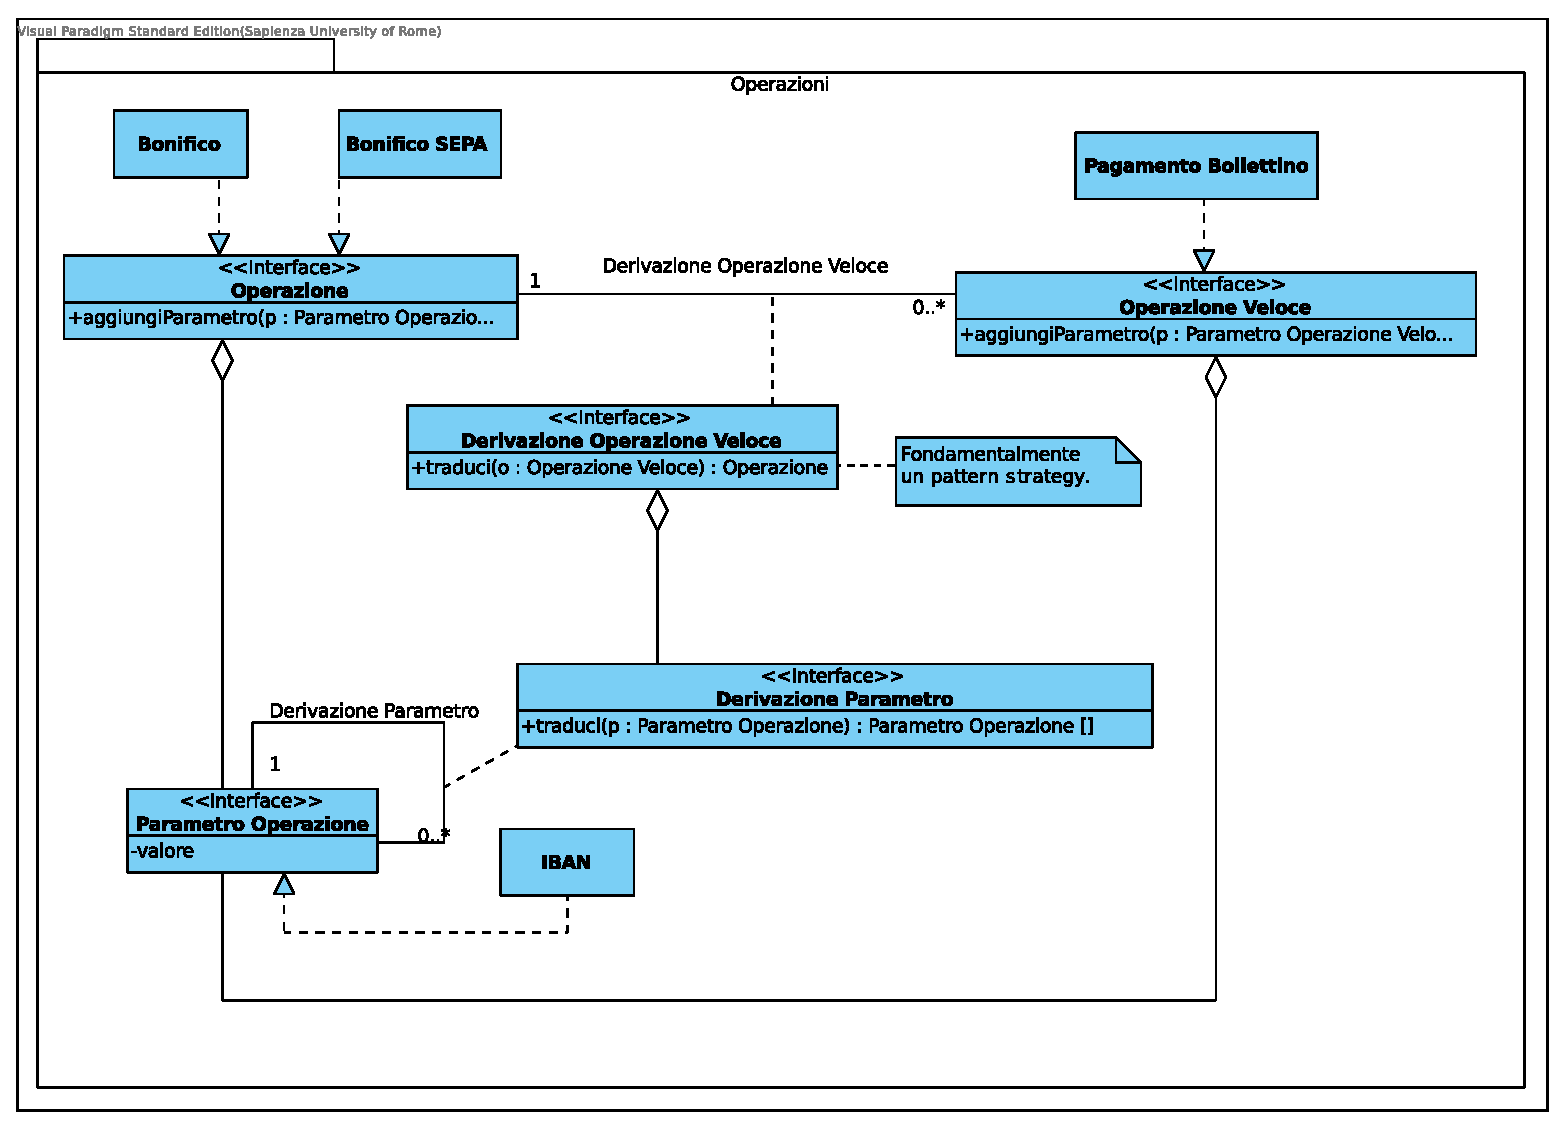
\includegraphics[width=\textwidth]{Images/Operazioni.eps}
	\caption{Classi per la gestione delle operazioni ordinarie e delle operazioni veloci.}
	\label{fig:operazioni}
\end{figure*}

Il sistema di traduzione da Operazione Veloce a Operazione (ordinaria) avviene attraverso una collezione di \emph{meccanismi} di traduzione, ossia di algoritmi di mapping dai parametri delle Operazioni Veloci ai parametri delle Operazioni ordinarie.

Un meccanismo di mapping comune consiste nella traduzione diretta di un parametro di Operazione Veloce in un parametro di Operazione ordinaria, ad esempio la traduzione del nome di una compagnia elettrica nell'IBAN della stessa.
